% Write about states and density matrices
% Add appendix about the JC interaction Hamiltonian and sisspertion
% Add appendix about quantum optics, coherent states, fock states

\documentclass{article}
\usepackage[utf8]{inputenc}
\usepackage{physics}
\usepackage{appendix}
\usepackage{amsfonts}
\usepackage{color} 
\usepackage{textcomp}
\usepackage[T1]{fontenc, url}
\usepackage{titlesec}
\setcounter{secnumdepth}{4}
\usepackage{multirow}
\usepackage{minted} % Code highlighting
\usepackage{adjustbox}
\usepackage{graphicx}
\usepackage{amsmath, amssymb, amsthm} % Mathematical packages
\usepackage{parskip} % Removing indenting in new paragraphs
\urlstyle{sf}
\usepackage{color}
\usepackage{subcaption} 
\usepackage{appendix}
\usepackage{chngcntr} % needed for correct table numbering
\counterwithin{table}{section} % numbering of tables 
\counterwithin{figure}{section} % numbering of figures
\numberwithin{equation}{section} % numbering of equations
\hyphenpenalty=100000 % preventing splitting of words
\sloppy 
\raggedbottom 
\usepackage{xparse,nameref}
\usepackage[bottom]{footmisc} % Fotnotes are fixed to bottom of page
\usepackage{lipsum} % For genereating dummy text
\usepackage{hyperref}
\hypersetup{
    colorlinks,
    citecolor=black,
    filecolor=black,
    linkcolor=black,
    urlcolor=black
}

\usepackage[margin=2.54cm]{geometry} % sets margins for the document
\usepackage{setspace}
\linespread{1.5} % line spread for the document
\usepackage{microtype}

\titleformat*{\section}{\LARGE\bfseries} % \section heading
\titleformat*{\subsection}{\Large\bfseries} % \subsection heading
\titleformat*{\subsubsection}{\large\bfseries} % \subsubsection heading

\titleformat{\paragraph}
{\normalfont\normalsize\bfseries}{\theparagraph}{1em}{}
\titlespacing*{\paragraph}
{0pt}{3.25ex plus 1ex minus .2ex}{1.5ex plus .2ex}


% ----- Figures and tables ----- 
\usepackage{fancyhdr}
\usepackage{subfiles}
\usepackage{array}
\usepackage[rightcaption]{sidecap}
\usepackage{wrapfig}
\usepackage{float}
\usepackage[labelfont=bf]{caption} % bold text for captions
\usepackage[para]{threeparttable} % fancy tables, check these before you use them
\usepackage{url}
\usepackage[table,xcdraw]{xcolor}
\usepackage{makecell}
\usepackage{hhline}


% ----- Sources -----
\usepackage{natbib}
\bibliographystyle{apa} % citation and reference list style
\def\biblio{\clearpage\bibliographystyle{apa}\bibliography{References.bib}} % defines the \biblio command used for referencing in subfiles - DO NOT CHANGE


% ----- Header and footer -----
\pagestyle{fancy}
\fancyhead[R]{\thepage} % page number on right for odd pages and left for even pages in the header
\fancyhead[L]{\nouppercase{\rightmark}} % chapter name and number on the right for even pages and left for odd pages in the header
%\renewcommand{\headrulewidth}{0pt} % sets thickness of header line
\fancyfoot{} % removes page number on bottom of page


% ----- Header of the frontpage ----- 
\fancypagestyle{frontpage}{
	\fancyhf{}
	\renewcommand{\headrulewidth}{0pt}
	\renewcommand{\footrulewidth}{0pt}
	\vspace*{1\baselineskip}
	
	\fancyhead[C]{Project for The Open University of Israel
	\linebreak       Done at The Weizmann Institute of Science\vspace*{5\baselineskip}}
	\fancyhead[L]{ 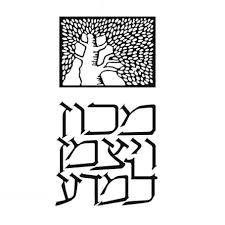
\includegraphics[width=1.2in]{Logo.png}}
	\fancyhead[R]{ 
\includegraphics[width=1.2in]{OpenLogo.jpg}}
}


%-----------------------------------------------------

%\title{Controlling a Superconducting Quantum Computer}
%\author{Daniel Cohen Hillel}
%\date{}

\begin{document}

\def\biblio{} % resets the biblio command, if not here a new reference list will be produced after every chapter

\begin{titlepage}
	
	\newgeometry{top=1 in, bottom=1 in, left=1 in, right= 1 in} 
	
	\thispagestyle{frontpage}
	
	\begin{center}
		
		\vspace*{6\baselineskip}
	
		
		{\Large \textbf{Controlling a Superconducting Quantum Computer\\}}
		
        \vspace*{1,5\baselineskip}

		\large{\textbf{Daniel Cohen Hillel}}\\
		\large{\textbf{Supervisor: Dr. Serge Rosenblum}}\\
		
		\vspace{1,5\baselineskip}
		
		\large{Advanced Project in Physics A (20382)}\\
		\large{The Open University of Israel}\\
		
		\vspace{1,5\baselineskip}
		\large{The Weizmann Institute}\\

	\end{center}
	
\end{titlepage}
\restoregeometry % restores the margins after frontpage
%\nocite{*} % uncomment if you want all sources to be printed in the reference list, including the ones which are not cited in the text 

\pagenumbering{gobble} % suppress page numbering
\thispagestyle{plain} % suppress header

%\maketitle

\newpage

\tableofcontents

\newpage
\pagenumbering{arabic}
\section{Introduction}

\subsection{What is a Quantum Computer?}
We'll assume the reader understands the basics of computing and quantum mechanics, here's a brief overview. \newline
 A classical computer is, essentially, a calculator, not of "Regular" numbers but of \textit{binary numbers} \footnote{ add further reading about binary numbers}. A \textit{binary digit}("\textit{bits}" from now on) can be in one of two states, usually represented by 0 and 1. We can use \textit{logic gates} to control and manipulate bits to do all kinds of calculations\footnote{Additional information about bit calculation}. This is the building blocks of the classical computer, with the ability to do calculation with bits, and the ability to store bits in the memory we are able to construct a computer.\newline \par
So what is a quantum computer then? Well, if the classical computer uses bits to do calculations, a quantum computer uses \textit{quantum bits}("\textit{qubits}" from now on) for it's calculations. A qubit, much the same as a bit, has 2 states, a 0 state and a 1 state(notated $\ket{0}$ and $\ket{1}$ for reasons we'll see later), the difference is that a qubit can be in a \textit{superposition} of the 2 states, so the qubit has essentially and infinite amount of possible states

\subsection{Qubits and Quantum Gates}

\subsection{Algorithms and Further motivation}

\subsection{Superconducting Quantum Computers}

\newpage
\section{Our System}

\subsection{The cavity}

\subsection{The Transmon}

\subsection{The Oscillator}

\subsection{Describing the System Mathematically}  % Metntion the JC model
To describe the system mathematically we are going to calculate it's Hamiltonian, that way we can run simulations of the system with the Schrodinger equation.\par
We can partition the system into different parts and analyse each part individually, so the total system Hamiltonian will be:

\begin{equation}
H(t) = H_{Oscillator} + H_{Transmon}+ H_{Interaction} + H_{Drive}(t)
\end{equation}

We'll begin by the easy to characterize, Transmon And Oscillator, they are a simple quantum system that can be described by the uppering and lowering operators \footnote{See appendix A}. We can write:
\begin{equation}
H_{Oscillator} = \omega_C a^\dag{}a
\end{equation}
\begin{equation}
H_{Transmon} = \omega_T b^\dag{}b
\end{equation}
We can find $\omega_C$ and $\omega_T$ experementally. % Maybe add a few words about how to do so and about the fact that this is only an harmonic approximation
\par
The next part to characterize is the interaction(See appendix A), again by the Jaynes–Cummings model, we can write the interaction hamiltonian as:
\begin{equation}
H_{Interaction} = \chi a^\dag{} a  b^\dag{} b % Again, this is only an harmonic approximation
\end{equation}
Again, we can measure $\chi$ experimentally.  % Maybe add more about how it's done
\par
Finally, we can characterize the driven and most important part of the system. It can be written as: % Add more about how do you get to that equation. Is it from Maxwell?

\begin{equation}
H_{Drive} = \epsilon_C(t)a + \epsilon_T(t)b + h.c.
\end{equation}
Or as(expanding the hermitian conjurgate):

\begin{equation}
H_{Drive} = \epsilon_{I_C}(t)(a + a^\dag{}) + \epsilon_{Q_C}(t)(a - a^\dag{})i + \epsilon_{I_T}(t)(b + b^\dag{})+ \epsilon_{Q_T}(t)(a - a^\dag{})i
\end{equation}

\newpage
\section{Optimal Control}

\subsection{What's GRAPE} % Add imagery of a step-wise constant function
As explained in previous sections, to control our qubit and manipulate it, we need to send microwave pulses in the cavity. The problem is, what pulse do we send? How does it look? sin? cos? In what frequency? or maybe even some arbitrary wave. \par
To answer this question, we can model our system on a normal computer and simulate what happens when you send a pulse, then, we can try to change the pulse(in a smart way) until we get the desired effect. So for example, let's say we want to find the wave pulse that corresponds to the NOT gate, we can start by guessing some random wave(constant zero, sin and so on), the random wave probably won't act as a NOT gate, then, we change the wave a little bit many times and on each iteration the pulse acts more and more as a NOT gate.\par
So what's GRAPE than? The *GR*adient *A*scent *P*ulse *E*ngineering was first proposed in [2]. When we model our system, we treat the wave as a step-wise constant function, so the wave is just an array with many variables and we want to find the best values that give the result that we want. then we set a cost function \footnote{discussed in details in the next section} that tells us how are the values of the wave to give the wanted result. This cost function is a many dimensional function(each step of the wave is a dimension of the cost function), and we can find its gradient. Using the cost function and it's gradient we can use some optimization algorithm(mainly, the L-BFGS-B method) to find the maximum of the cost function that gives us the optimal wave to send to the cavity.

\subsection{The Cost Function}
So what is this cost function really? \textit{\textbf{Fidelity}}. It measures the "closeness" of two quantum states and varies between 0 and 1. So for example, the fidelity between state $\ket{0}$ and state $\ket{1}$ is equal to 0, because they are the most different two quantum states can be, while for example the fidelity between state $\ket{0}$ and state $\ket{0}$ is equal to 1, because they are the closest two states can be to each other(for a matter of fact, every state has fidelity 1 with itself and end fidelity 0 with an opposite state). But still, how do we calculate the fidelity between two states? well, turns out its very simple, it's just their product \footnote{Assuming both states are pure states}. We can write:

\begin{equation}
F(\psi_1, \psi_2) = \abs{\braket{\psi_1}{\psi_2}}^2
\end{equation}
We want to maximize the fidelity with GRAPE.\par
In a previous chapter we characterized the Hamiltonian of the system(equation (num)), so now we can use the good old \textit{time-dependent Schrodinger equation}:

\begin{equation}
i\hbar\frac{d}{dt}\ket{\Psi(t)} = \hat{H}\ket{\Psi(t)}
\end{equation}

And also, the Hamiltonian of the system is in the form\footnote{Further details were given in section 2.4}:

\begin{equation}
H(t) = H_0 + \sum_k{\epsilon_k(t) H_k} % Maybe put the next part before the part about the Schrodinger equation
\end{equation}

Because of the way this Hamiltonian is built, on each constant step of the wave function, the Hamiltonian is constant, and luckily for us, the solution of the Schrodinger equation for a constant Hamiltonian is pretty simple and given by\footnote{Add a simple justification}

\begin{equation}
U(t) = e^{-\frac{i}{\hbar}\int_{T_0}^{T_1}H(t)dt}
\end{equation}

And because we chose $T_0$ and $T_1$ as the end points of a step of the functions, the total Hamiltonian of the system is constant so the integral is just a simple multiplication by $T_1-T_0$ which we'll write as $\delta t$. So the solution is
\begin{equation}
U(t) = e^{-\frac{i\cdot \delta t}{\hbar}H(t)}
\end{equation}
More then that, to solution over all time is the product of all the solutions for each constant piece. So 
\begin{equation}
U(\epsilon(t)) = \prod_{k = 1}^NU_k
\end{equation}
Where N is the number of time steps in the simulation(larger N is a more precise simulation). \par
This way the state of the qubit after the drive is given by:
\begin{equation}
\ket{\Psi_{final}} = U\ket{\Psi_{initial}}
\end{equation}
This way if we want to calculate the fidelity after applying the drives we can simply calculate the fidelity between the wanted state and the final state,
\begin{equation}
F(\Vec{\epsilon(t)}) = F(\Psi_{target}, \Psi_{final}) = \abs{\bra{\Psi_{target}}U\ket{\Psi_{initial}}}^2
\end{equation}
m
Now, theoretically we can use an algorithm to try different waves until we find a wave that does what we want(brute force for example), but this will take to much time and the computation won't finish in any reasonable amount of time. Because of this, we'll want to use a smart search algorithm(such as L-BFGS-B) but to do so we need the gradient of the cost function(the variables of the cost function are the values of the steps of the drive pulses). We can obviously use the finite difference method to calculate the gradient but this method is heavy on the computation and has a lot of over head. We'll take a smarter approach to calculating the gradient.\par
We can look at the expression,  % Needs to go over this

\begin{equation}
c = \braket{\Psi_{target}}{\Psi_{final}} = \bra{\Psi_{target}}U\ket{\Psi_{initial}}
\end{equation}

We want to differentiate this expression by each control parameter. U is defined as:

$$U = U_N U_{n-1}...U_2 U_1$$

And when differentiating by a control parameter only one $U_k$ is affected, so we can write,

$$\frac{dc}{d\epsilon_k} = \bra{\Psi_{target}}U_N U_{N-1}...\frac{dU}{d\epsilon_k}...U_2 U_1\ket{\Psi_{initial}} $$

Assuming very small time steps we can derive $U_k$ over $\epsilon_k$,

$$U_k = e^{-\frac{i\cdot \delta t}{\hbar}H(t)}$$
$$\frac{dU_k}{d\epsilon_k} = \frac{i \delta t}{\hbar}\frac{dH}{d\epsilon_k} U_k$$

We can use this expression as the gradient values but it's still rather complex computationally($N^2$ complexity).\par
We can use a bit different method to calculate the gradient to save on the computation by reducing the overhead.


\subsection{Constraints}

\newpage
\section{Controlling the FPGA(wave generator)}
\newpage
\section{Conclusion}


\newpage

\appendix
\section{The Jaynes–Cummings Model}
Our goal is to mathematically model the Hamiltonian of a system of a two-level atom interacting with a single quantized mode of an optical cavity's electromagnetic field. %Add details about the original paper by Edwin Jaynes and Fred Cummings
\par
First we'll divide the system into 3 parts, The atom(it can be other two-level quantum systems), the cavity(electromagnetic field with quantized modes) and the interaction between the atom and the cavity(an atom can emit a photon to the cavity and change it's electromagnetic field, or catch a photon from the cavity and go up an energy level).\par  % http://aliramadhan.me/files/jaynes-cummings-model.pdf
Let's start with the cavity(we'll consider a one dimensional cavity for now). 
\subsection{The Homogeneous Electromagnetic Wave Equations}
Maxwell's equations in free space are:

\begin{equation}
    \label{eq:Maxwell-1}
    \grad \cdot \textbf{E} = 0
\end{equation}
\begin{equation}
    \label{eq:Maxwell-2}
    \grad \cdot \textbf{B} = 0
\end{equation}    
\begin{equation}
    \label{eq:Maxwell-3}
    \grad \cross \textbf{E} = \frac{\partial\textbf{B}}{\partial t}
\end{equation}
\begin{equation}
    \label{eq:Maxwell-4}
    \grad \cross \textbf{B} = \mu_0 \epsilon_0 \frac{\partial\textbf{E}}{\partial t}
\end{equation}

Taking the curl of \ref{eq:Maxwell-3} and \ref{eq:Maxwell-4} we get
\begin{equation}
    \label{eq:curl-E}
    \curl{(\curl{\textbf{E}})} = \curl{(-\frac{\partial \textbf{B}}{\partial t})} = -\frac{\partial}{\partial t}(\curl{\textbf{B}}) = - \mu_0 \epsilon_0 \frac{\partial^2 E}{\partial t^2}
\end{equation}
\begin{equation}
    \label{eq:curl-B}
    \curl{(\curl{\textbf{B}})} = \curl{(\mu_0 \epsilon_0 \frac{\partial E}{\partial t})} = \mu_0 \epsilon_0\frac{\partial}{\partial t}(\curl{E}) = - \mu_0 \epsilon_0 \frac{\partial^2 \textbf{B}}{\partial t^2}
\end{equation}
   
We can use the vector identity
\begin{equation}
    \nabla \times \left( \nabla \times \mathbf{V} \right) = \nabla \left( \nabla \cdot \mathbf{V} \right) - \nabla^2 \mathbf{V}
\end{equation}
And obtain from \ref{eq:curl-E} and \ref{eq:curl-B}
\begin{equation}
    \nabla(\nabla \cdot \textbf{E}) - \nabla^2 \textbf{E} = -\mu_0\epsilon_0\frac{\partial^2 \textbf{E}}{\partial t^2}
\end{equation}
\begin{equation}
    \nabla(\nabla \cdot \textbf{B}) - \nabla^2 \textbf{B} = -\mu_0\epsilon_0\frac{\partial^2 \textbf{B}}{\partial t^2}
\end{equation}
Now, we can use \ref{eq:Maxwell-1} and \ref{eq:Maxwell-2} To cancel the left most term and get
\begin{equation}
    \nabla^2 \textbf{E} = \mu_0\epsilon_0\frac{\partial^2 \textbf{E}}{\partial t^2}
\end{equation}
\begin{equation}
    \nabla^2 \textbf{B} = \mu_0\epsilon_0\frac{\partial^2 \textbf{B}}{\partial t^2}
\end{equation}
Now because we know that $v_{ph} = \frac{1}{\sqrt{\mu_0\epsilon_0}}$ and that the phase velocity of electromagnetic waves in a vacuum is the speed of light, $c_0$, we get

\begin{equation} \label{eq:Homo_electro_wave}
    \begin{split}
        \nabla^2 \textbf{E} = \frac{1}{c_0^2}\frac{\partial^2 \textbf{E}}{\partial t^2} \\
        \nabla^2 \textbf{B} = \frac{1}{c_0^2}\frac{\partial^2 \textbf{B}}{\partial t^2}
    \end{split}
\end{equation}
% Check these equations with serge
These equation are called \textit{the homogeneous electromagnetic wave equations}.
We'll pick a polarization arbitrarily to be in the x direction(that way we get only the component of the electric field and the y component of the magnetic field, $E_x$ and $B_y$) so now we get,
\begin{equation} \label{eq:Homo_electro_wave_pol}
    \begin{split}
        \frac{\partial^2 E_x}{\partial x^2} = \frac{1}{c_0^2}\frac{\partial^2 E_x}{\partial t^2} \\
        \frac{\partial^2 B_y}{\partial y^2} = \frac{1}{c_0^2}\frac{\partial^2 B_y}{\partial t^2} 
    \end{split}
\end{equation}
\subsection{The Hamiltonians}
We can easily solve \ref{eq:Homo_electro_wave_pol} using separation of variables,
$$E_x(z, t)= Z(z)T(t)$$
Yielding the solution,
\begin{equation}
    \begin{split}
        E_x(z, t) = \sqrt{\frac{2 \omega_c^2}{V \epsilon_0}}q(t)\sin{kz} \\
        B_y(z, t) = \sqrt{\frac{2 \mu_0}{V}}\dot{q}(t)\cos{kz}
    \end{split}
\end{equation}
where $V$ is the effective volume of the cavity, $q$ is a time-dependent amplitude with units of length, and $k = m\pi/L$ for
an integer $m > 0$

The Hamiltonian is given by
\begin{equation}
    \begin{split}
        H = \frac{1}{2}\int\epsilon_0 \textbf{E}^2 + \frac{\textbf{B}^2}{\mu_0} dV \\
        = \frac{1}{2}\int\epsilon_0 E_x^2(z, t) + \frac{B_y^2(z, t)}{\mu_0} dz \\
        = \frac{1}{2}[\dot{q}^2(t) + \omega_c^2 q^2(t)]
    \end{split}
\end{equation}
This looks like the Hamiltonian of an harmonic oscillator.

Now, going from dynamical variables to operators(considering $\dot{q} \equiv p$) we get,
\begin{equation}
    \begin{split}
         \hat{E}_x(z, t) = \sqrt{\frac{2 \omega_c^2}{V \epsilon_0}}\hat{q}(t)\sin{kz} \\
         \hat{B}_y(z, t) = \sqrt{\frac{2 \mu_0}{V}}\hat{p}(t)\cos{kz} \\
         \hat{H} = \frac{1}{2}[\hat{p}^2(t) + \omega_c^2 \hat{q}^2(t)]
    \end{split}
\end{equation}

Let’s introduce creation and annihilation operators,
$$\hat{a}(t) = \frac{1}{\sqrt{2\hbar\omega_c}}[\omega_c\hat{q}(t) + i\hat{p}(t)]$$
$$\hat{a}^\dag(t) = \frac{1}{\sqrt{2\hbar\omega_c}}[\omega_c\hat{q}(t) - i\hat{p}(t)]$$

We can write the electric and magnetic field as,
\begin{equation}
    \begin{split}
         \hat{E}_x(z, t) = E_0[\hat{a}(t) + \hat{a}^\dag(t)]\sin{kz} \\
         \hat{B}_y(z, t) = \frac{E_0}{c}[\hat{a}(t) - \hat{a}^\dag(t)]\cos{kz}
    \end{split}
\end{equation}
And we can write the Hamiltonian as,
\begin{equation}
    \hat{H} = \hat{H}_{cavity} = \hbar\omega_c[\hat{a}\hat{a}^\dag + \frac{1}{2}] \approx \hbar\omega_c\hat{a}\hat{a}^\dag
\end{equation}
We can ignore the zero-point energy $\frac{\hbar\omega_c}{2}$ if we define it as the zero energy point.

Now that we have the cavity's Hamiltonian, we can go on to calculate the atom(qubit) Hamiltonian. \newline
Remember that the qubit is a 2-level system, meaning we can define it has a superposition of the ground, $\ket{g}$, and excited, $\ket{e}$, states. The energy of the atom is the sum of the energy of each state times it's energy($\sum E_sP(\ket{s})$). The probabilty to be in a state $\ket{s}$ is given by $\ket{s}\bra{s}$ so we can write,
\begin{equation}
    \hat{H}_{atom} = E_g\ket{g}\bra{g} + E_e\ket{e}\bra{e}
\end{equation}
Using the vector representation of these states we'll write,
%\begin{equation}
    \begin{align*} 
        \hat{H}_{atom} &= 
        E_e \begin{bmatrix}
        1 & 0     \\
        0   & 0   \\
        \end{bmatrix}
        + E_g \begin{bmatrix}
        0 & 0     \\
        0   & 1   \\
        \end{bmatrix} = 
        \begin{bmatrix}
        E_e & 0     \\
        0   & E_g   \\
        \end{bmatrix} \\
        &= \frac{1}{2}\begin{bmatrix}
        E_g + E_e & 0          \\
        0         & E_g + E_e  \\
        \end{bmatrix} +
        \frac{1}{2}\begin{bmatrix}
        E_e - E_g & 0          \\
        0         & -(E_e - E_g)  \\
        \end{bmatrix} \\
        &= \frac{1}{2}(E_g + E_e)\begin{bmatrix}
        1 & 0          \\
        0         & 1  \\
        \end{bmatrix} +
        \frac{1}{2}(E_e - E_g)\begin{bmatrix}
        1 & 0          \\
        0         & -1  \\
        \end{bmatrix} \\
        &= \frac{1}{2}(E_g + E_e)\mathbb{I} + \frac{1}{2}(E_e - E_g)\hat{\sigma}_z
    \end{align*}
%\end{equation}
Again, we can define the zero point energy so that the first term becomes $0$. We know the difference between the excited state energy and the ground state energy because it's approximately an harmonic osscilator so $E_e - E_g = \hbar\omega_a$ where $\omega_a$ is the atom frequancy. Now we can write,
\begin{equation}
    \hat{H}_{atom} = \frac{1}{2}\hbar\omega_a\hat{\sigma}_z
\end{equation}

\subsection{The Dispersive Limit}


\end{document}
